% --------------------------------------
% Document Class
% --------------------------------------
\documentclass[a4paper,11pt]{article}
% --------------------------------------



% --------------------------------------
% Use Package
% --------------------------------------

\usepackage[francais]{babel}
\usepackage{ucs}
\usepackage[utf8]{inputenc}
\usepackage[T1]{fontenc}

\usepackage{makeidx}
\usepackage{color}
\usepackage{graphicx}
\usepackage{float}
\usepackage[hidelinks]{hyperref} 
\usepackage{geometry}
%\usepackage{lastpage}
%\usepackage{marginnote}
\usepackage{fancyhdr}
%\usepackage{titlesec}
%\usepackage{framed}
\usepackage{amsmath}
\usepackage{empheq}
\usepackage{array}
\usepackage{multicol}
\usepackage{csquotes}
%\usepackage{adjustbox}

% insert code
\usepackage{listings}

% define our color
\usepackage{xcolor}

% code color
\definecolor{ligthyellow}{RGB}{250,247,220}
\definecolor{darkblue}{RGB}{5,10,85}
\definecolor{ligthblue}{RGB}{1,147,128}
\definecolor{darkgreen}{RGB}{8,120,51}
\definecolor{darkred}{RGB}{160,0,0}

% other color
\definecolor{ivi}{RGB}{141,107,185}

\def\verticaltext#1{\rotatebox[origin=c]{90}{\x{#1}}}


\lstset{
    language=python,
    captionpos=b,
    extendedchars=true,
    frame=lines,
    numbers=left,
    numberstyle=\tiny,
    numbersep=5pt,
    keepspaces=true,
    breaklines=true,
    showspaces=false,
    showstringspaces=false,
    breakatwhitespace=false,
    stepnumber=1,
    showtabs=false,
    tabsize=3,
    basicstyle=\small\ttfamily,
    backgroundcolor=\color{ligthyellow},
    keywordstyle=\color{ligthblue},
    morekeywords={include, printf, uchar},
    identifierstyle=\color{darkblue},
    commentstyle=\color{darkgreen},
    stringstyle=\color{darkred},
}


% --------------------------------------



% --------------------------------------
% Page setting
% --------------------------------------
%\pagestyle{empty}
\setlength{\headheight}{15pt}

\setcounter{secnumdepth}{3}
\setcounter{tocdepth}{2}

\makeatletter
\@addtoreset{chapter}{part}
\makeatother 

\hypersetup{       % parametrage des hyperliens
  colorlinks=true,  % colorise les liens
  breaklinks=true,  % permet les retours à la ligne pour les liens 
                    % trop longs
  urlcolor= blue,   % couleur des hyperliens
  linkcolor= black, % couleur des liens internes aux documents 
                    % (index, figures, tableaux, equations,...)
  citecolor= green  % couleur des liens vers les references 
                    % bibliographiques
}

% --------------------------------------

% --------------------------------------
% Information
% --------------------------------------
\title{
  \noindent\hrulefill \\
  \vspace{10mm}
  \textbf{Compte-rendu VisA} \\
  \vspace{5mm}
  TP: Approche de la logique floue.
}

\author{Gaëtan DEFLANDRE}
% --------------------------------------

\definecolor{myColor}{rgb}{0.5, 0.1, 0.75}

% --------------------------------------
% Begin content
% --------------------------------------
\begin{document}

\maketitle
\noindent\hrulefill \\


\section*{Introduction}

Les techniques de segmentation comme le clustering permettent de 
calculer des classes d'appartenance. Ces classes permettent de 
décrire les pixels de l'image de manière net et sans ambiguïté.\\

Or, ce type d'approche n'est pas toujours évident. Dans cette 
configuration, un pixel appartient ou pas à une classe. La logique 
floue permet d'éviter ce genre de segmentation trop net, avec 
fonction d'appartenance qui donne des facteurs plutôt que des 
valeurs booléennes.\\


\newpage


\section{Fonctions d'appartenance}

Soit les sous-ensembles flous correspondant aux températures basses, 
moyennes et hautes.

\begin{figure}[H]
  \begin{center}
  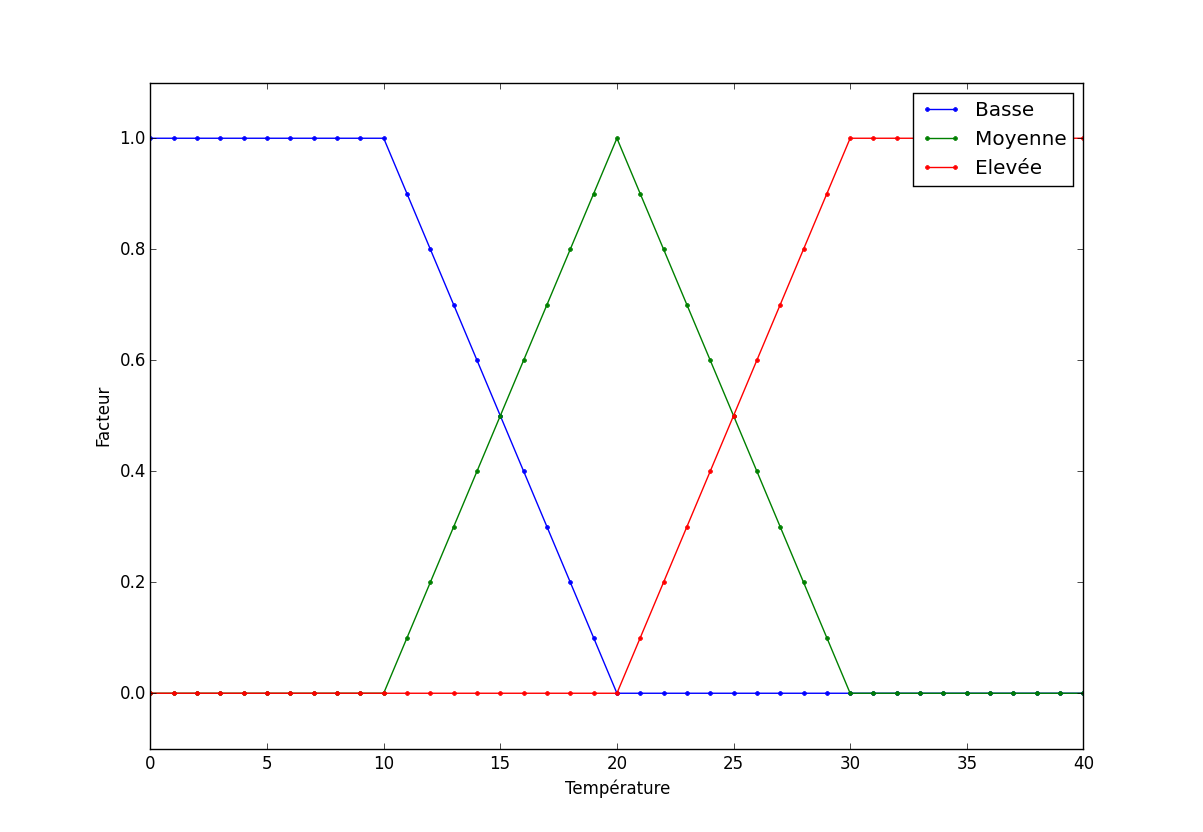
\includegraphics[height=280px]{images/exercice1.png}
  \caption{Les fonctions d'appartenance.}
  \end{center}
\end{figure}

Voici, le tableau qui montre les degrés d'appartenance aux différentes 
fonctions pour une température de 16\degre C.

\begin{table}[H]
  \begin{center}
    \begin{tabular}{|l|c|}
      \hline
       & Degrés d'appartenance \\
      \hline
      \hline
      Temp basse & 0.4 \\
      \hline
      Temp moyenne & 0.6 \\
      \hline
      Temp elevée & 0.0\\
      \hline
    \end{tabular}
    \caption{Degrés d'appartenance pour une température de 16\degre C}
  \end{center}
\end{table}


\newpage

\section{Opérateurs de la logique floue}

Maintenant, nous allons voir l'opérateur min qui donne le sous-ensemble 
flou minimum entre deux fonctions floues. Voici par exemple le 
minimum entre la fonction de températures basses et moyennes.

\begin{figure}[H]
  \begin{center}
  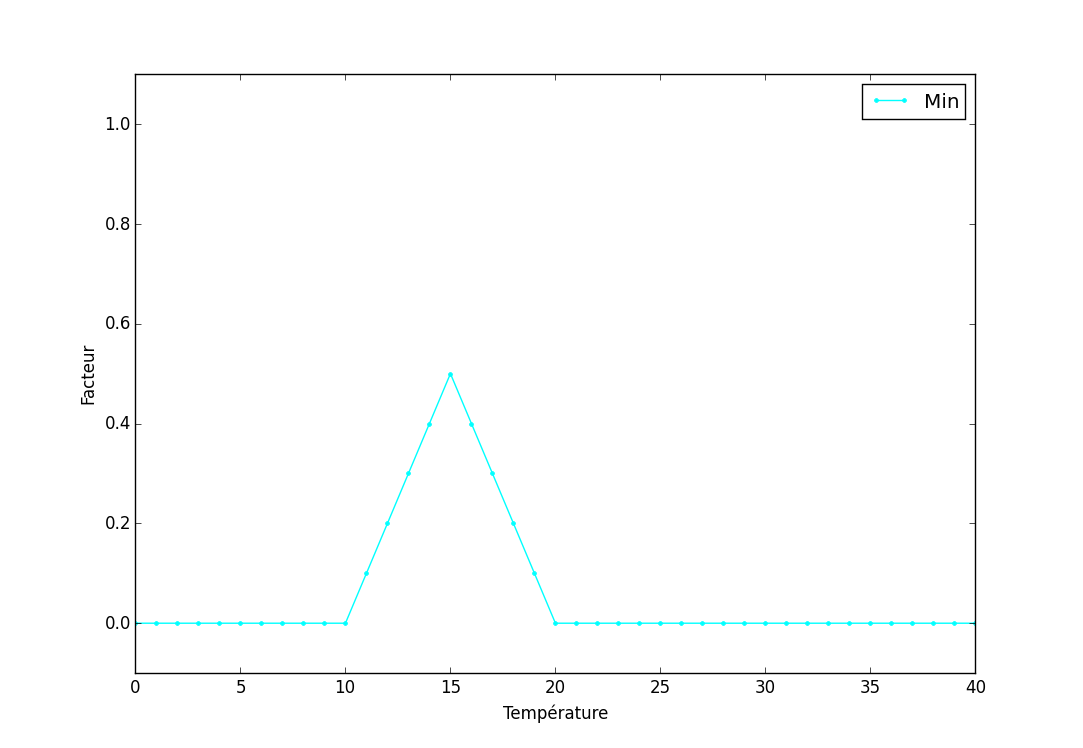
\includegraphics[height=280px]{images/min.png}
  \caption{Fonction minimum entre la fonction de températures basses et moyennes.}
  \end{center}
\end{figure}

Ensuite, l'opérateur max donne le sous-ensemble flou maximum 
entre deux fonctions floues. Par exemple le maximum entre la 
fonction de températures moyennes et hautes.

\begin{figure}[H]
  \begin{center}
  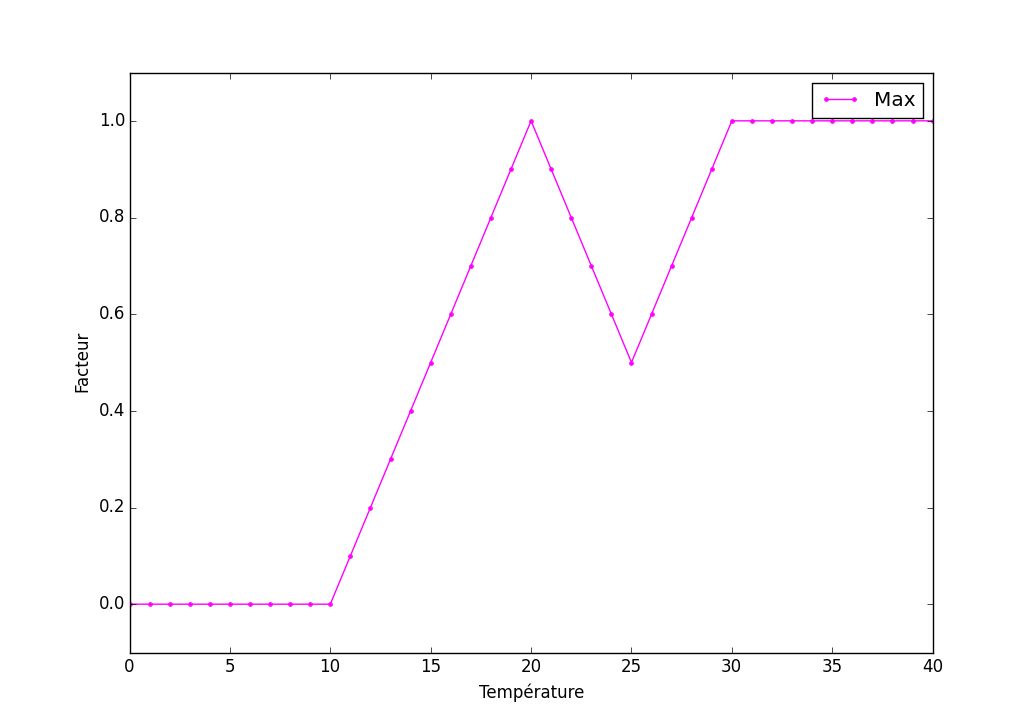
\includegraphics[height=280px]{images/max.png}
  \caption{Fonction maximum entre la fonction de températures moyennes et hautes.}
  \end{center}
\end{figure}

\newpage

\section{Implication floue}

Pour finir ce TP, nous utilisons les règles floues. Elles 
permettent, à partir d'une température d'entrée, de déterminer 
la puissance de chauffe en utilisant une implication de Mamdani.\\

Nous travaillons avec la règle suivante: SI <<Température basse>> 
ALORS <<Chauffer fort>>. Sous-ensemble flou <<Chauffer fort>> est 
représenté par la figure ci-dessous.

\begin{figure}[H]
  \begin{center}
  \includegraphics[height=280px]{images/heat.png}
  \caption{Sous-ensemble flou <<Chauffer fort>>}
  \end{center}
\end{figure}

Pour calculer l'implication floue, pour la règle précédente, 
nous utilisons la méthode de Mamdani.\\

Pour une température de 12\degre C, il faut calculer le degré 
d'appartenance à la fonction flou <<Température basse>>. Nous 
obtenons une valeur en $y$ de 0,8 qui ne doit pas être dépassé.\\

Enfin, il faut résoudre la fonction affine <<Chauffer fort>> pour 
déterminer la puissance de chauffe. L'équation de cette fonction 
est :
$$
f(x)=\frac{1}{2}x-4
$$

D'où, nous pouvons déterminer la puissance de chauffe avec le 
calcul suivant:

$$
x = (y+4) * 2
$$

Donc la puissance de chauffe pour une température de 12\degre C 
est 9,6 KW.

\begin{figure}[H]
  \begin{center}
  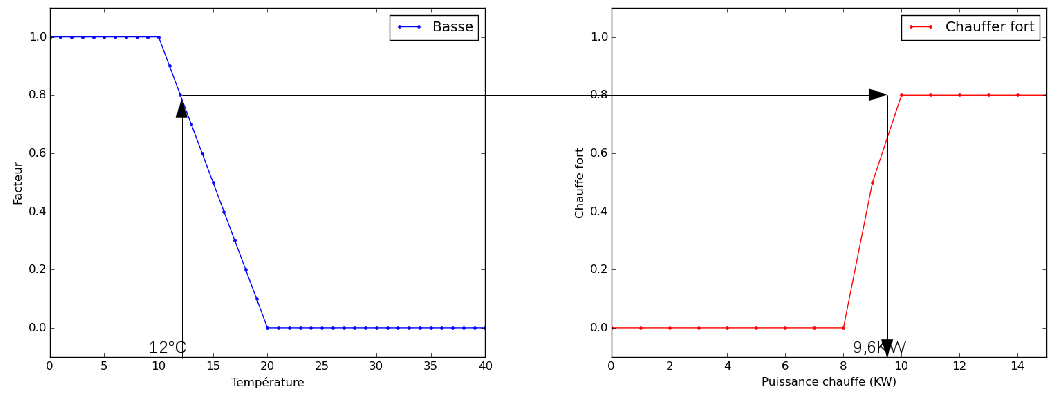
\includegraphics[height=170px]{images/low_mamdani_arrow.png}
  \caption{Fonction de températures basses et implication floue.}
  \end{center}
\end{figure}



\end{document}
